\documentclass
  [hyperref={colorlinks = true,linkcolor = blue, 
             citecolor = blue, urlcolor = blue}
  ]{beamer}

\setbeamertemplate{navigation symbols}{}
\setbeamertemplate{footline}[frame number]
 
\usepackage[utf8]{inputenc}

\usepackage[newfloat]{minted}

\usepackage{pgf}
\usepackage{tikz}
\usepackage{upquote}
\usepackage{natbib}
\usepackage[export]{adjustbox}
\usepackage{amsmath}
\usepackage{amssymb}
\usepackage{trfrac}

\usetikzlibrary{arrows,automata,fit, shapes.geometric}

\bibliographystyle{abbrvnat}

\newenvironment{code}{\captionsetup{type=listing}}{}
\SetupFloatingEnvironment{listing}{name=Listing}

\setbeamertemplate{items}[square]

\title{Enforcing a discipline of Total Functional Programming
through Dependent Types}
\author{Donovan Crichton}
  
\date{July 2024}

\begin{document}
 
\frame{\titlepage}

\begin{frame}[fragile]
  \frametitle{Preliminaries}
  \begin{itemize}
  \item Slides and Examples available at:
    \href{https://github.com/donovancrichton/Talks}
         {https://github.com/donovancrichton/Talks}
  \item This talk: BFPG/TotalFPThroughDepTypes
  \end{itemize}
\end{frame}

\begin{frame}[fragile]
\frametitle{About me}
\begin{minipage}[t]{\linewidth}
\noindent
  \begin{minipage}{0.5\linewidth}
    \begin{figure}[h]
       
\includegraphics[width=\linewidth]
         {Images/ANU.png}
    \end{figure}
  \end{minipage}
  \hfill
  \begin{minipage}{0.45\linewidth}
    \begin{itemize}
      \item 
        \href{https://cecc.anu.edu.au/people/donovan-crichton}
             {PhD Candidate}
      \item 
        \href{https://comp.anu.edu.au/research/clusters/computing-foundations/}
             {Computing Foundations}
      \item 
        \href{https://comp.anu.edu.au/}
             {School of Computing}
    \end{itemize}
  \end{minipage}
\end{minipage}
\hrule
  \begin{minipage}{0.5\linewidth}
    \begin{figure}[h]
      
\includegraphics[scale=0.5,width=\linewidth]
        {Images/GriffithLogo.png}
    \end{figure}
  \end{minipage}
  \hfill
  \begin{minipage}{0.45\linewidth}
  \begin{itemize}
    \item Visiting Scholar
    \item Trusted Systems Lab
    \item \href{https://www.griffith.edu.au/institute-integrated-intelligent-systems}{IIIS}
  \end{itemize}
  \end{minipage}
\hrule
  \begin{minipage}{0.5\linewidth}
    \begin{figure}[h]
      
\includegraphics[width=\linewidth]
        {Images/asd-logo.png}
    \end{figure}
  \end{minipage}
  \hfill
  \begin{minipage}{0.45\linewidth}
  \begin{itemize}
    \item ASD 
      \href{https://www.asd.gov.au/about/asd-anu-co-lab}{Co-Lab} 
      Scholar
  \end{itemize}
  \end{minipage}
\hrule
  \begin{minipage}{0.5\linewidth}
    \begin{figure}[h]
      
\includegraphics[width=\linewidth]
        {Images/VLClogo.png}
    \end{figure}
  \end{minipage}
  \hfill
  \begin{minipage}{0.45\linewidth}
  \begin{itemize}
    \item \href{https://veitchlister.com/}{Veitch Lister
    Consulting} 
    \item Software Engineer
  \end{itemize}
  \end{minipage}
\end{frame}

\begin{frame}[fragile]
\frametitle{Alex (I): A Lexer Generator Library (GHC)}
\setbeamercolor{block title}{fg=white,bg=purple!75!black}
\setbeamercolor{block body}{fg=black,bg=white!80!gray}
\begin{block}{Character Sets and Macros}
\begin{minted}{Bash}
-- character sets
$digit  = 0-9
$small  = a-z
$big    = A-Z
$dash   = \-
$gt     = \>
$prime  = \'
$uscore = \_
$lambda = \\
$idchar = [$small $big $digit $prime $uscore]
-- character set macros
@bigid   = big idchar*
@smallid = small idchar*
@arrow   = $dash $gt
\end{minted}
\end{block}
\end{frame}

\begin{frame}[fragile]
\frametitle{Alex (II): A Lexer Generator Library (GHC)}
\setbeamercolor{block title}{fg=white,bg=purple!75!black}
\setbeamercolor{block body}{fg=black,bg=white!80!gray}
\begin{block}{Regex Rules and Tokens}
\begin{minted}{Haskell}
-- <state>    <regex>   {<func>}
   <0>        @arrow    {tokArrow}
   <0>        @bigid    {tokBigId}
   <0>        @smallid  {tokSmallId}
   <0>        $lambda   {tokLambda}
{
  data Token = TSmallId | TBigId
    | TArrow | TLambda

  tokLambda :: input -> Alex Token
  tokLambda input = pure TLambda

  tokArrow :: input -> Alex Token
  tokArrow input = pure TArrow
}
\end{minted}
\end{block}
\end{frame}

\begin{frame}[fragile]
\frametitle{Alex (III): A Lexer Generator Library (GHC)}
\setbeamercolor{block title}{fg=white,bg=purple!75!black}
\setbeamercolor{block body}{fg=black,bg=white!80!gray}
\begin{block}{Output Token List}
\begin{minted}{Haskell}
  lex "\foo -> \bar -> \baz -> Baz foo bar"
-- gives us something like:
  [TLambda, TSmallId, TArrow, 
   TLambda, TSmallId, TArrow, 
   TLambda, TSmallId, TArrow,
   TBigId, TSmallId, TSmallId]
\end{minted}
\end{block}
\end{frame}

\begin{frame}[fragile]
\frametitle{Happy (I): A Parser Generator Library (GHC)}
\setbeamercolor{block title}{fg=white,bg=purple!75!black}
\setbeamercolor{block body}{fg=black,bg=white!80!gray}
\begin{block}{Token Directive: Mirrors the Lexer}
\begin{minted}{Haskell}
{
  import qualified Lexer as LEX
  import qualified ParseTree as AST
}
%token
  smallIdent {LEX.TSmallId}
  bigIdent   {LEX.TBigId}
  arrow      {LEX.TArrow}
  lambda     {LEX.TLambda}
\end{minted}
\end{block}
\end{frame}

\begin{frame}[fragile]
\frametitle{Happy (II): A Parser Generator Library (GHC)}
\setbeamercolor{block title}{fg=white,bg=purple!75!black}
\setbeamercolor{block body}{fg=black,bg=white!80!gray}
\begin{block}{Production Rules and Sadness}
\begin{minted}{Haskell}
Term :: {AST.Term}
  : smallIdent              {parseVar $1}
  | bigIdent                {parseDataCon $1}
  | lambda smallIdent
      arrow Term            {parseLambda $2 $4}
  | Term Term               {parseApp $1 $2}
{
  parseVar :: LEX.Token -> AST.Term
  parseVar (TSmallId) = MkSmallRef
  parseVar _          = ?whatgoeshere

  parseDataCon :: LEX.Token -> AST.Term
  parseDataCon (TBigId) = MkDataCon
  parseDataCon _        = ?whatabouthere?
}
\end{minted}
\end{block}
\end{frame}

\begin{frame}[fragile]
\frametitle{Awkward Pattern-Matches, A type is too large.}
A quick note on the Algebra of Types.
  \begin{minipage}{0.45\textwidth}
\setbeamercolor{block title}{fg=white,bg=orange!75!black}
\setbeamercolor{block body}{fg=white,bg=orange!25!black}
  \begin{block}{Types}
  $Unit = \{\ast\}$ \\
  $Bool = \{True, False\}$ \\
  $Pair(A, B) = A \times B$ \\
  $Either(A, B) = A \sqcup B$ \\
  $Maybe(A)     = \{\ast\} \sqcup A $\\
  $A \to B = A \mapsto B$
  \end{block}
  \end{minipage}
  \begin{minipage}{0.45\textwidth}
\setbeamercolor{block title}{fg=white,bg=green!75!black}
\setbeamercolor{block body}{fg=white,bg=green!25!black}
  \begin{block}{Cardinality}
  $|Unit|         = 1$ \\
  $|Bool|         = 2$ \\
  $|Pair(A, B)|   = |A| \times |B|$ \\
  $|Either(A, B)| = |A| + |B|$ \\
  $|Maybe(A)|     = 1 + |A|$ \\
  $|A \to B|      = |B|^{|A|}$
  \end{block}
  \end{minipage}
  
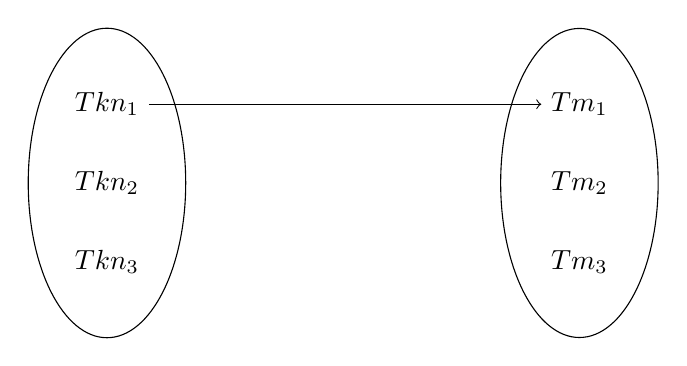
\begin{tikzpicture}
% Input Token
\node (Tkn1) at (0, 7) {$Tkn_1$};
\node[below of=Tkn1] (Tkn2) {$Tkn_2$};
\node[below of=Tkn2] (Tkn3) {$Tkn_3$};

% Output Term
\node (Tm1) at (6, 7) {$Tm_1$};
\node[below of=Tm1] (Tm2) {$Tm_2$};
\node[below of=Tm2] (Tm3) {$Tm_3$};

% arrows
\path[->] (Tkn1) edge (Tm1);
% set ellipses
\node[shape=ellipse,draw,minimum size=2cm,
      fit={(Tkn1) (Tkn3)}] {};
\node[shape=ellipse,draw,minimum size=2cm,
      fit={(Tm1) (Tm3)}] {};
\end{tikzpicture}
\end{frame}


\begin{frame}[fragile]
  \frametitle{Overview of Totality}
\setbeamercolor{block title}{fg=white,bg=green!75!black}
\setbeamercolor{block body}{fg=white,bg=green!25!black}
\begin{block}{Totality}
A function is total if it is \textit{defined over all
inputs}, and guaranteed to terminate.
\end{block}
\mintinline{haskell}{f :: Token -> Maybe Term}
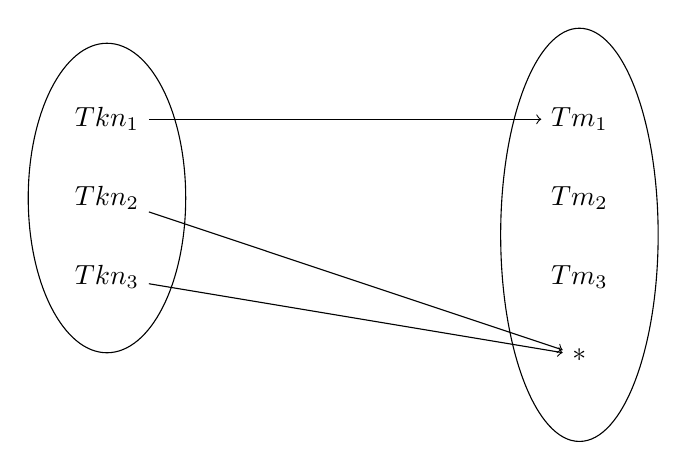
\begin{tikzpicture}
% Input Token
\node (Tkn1) at (0, 7) {$Tkn_1$};
\node[below of=Tkn1] (Tkn2) {$Tkn_2$};
\node[below of=Tkn2] (Tkn3) {$Tkn_3$};

% Output Term
\node (Tm1) at (6, 7) {$Tm_1$};
\node[below of=Tm1] (Tm2) {$Tm_2$};
\node[below of=Tm2] (Tm3) {$Tm_3$};
\node[below of=Tm3] (Nothing) {$\ast$};

% arrows
\path[->] (Tkn1) edge (Tm1);
\path[->] (Tkn2) edge (Nothing);
\path[->] (Tkn3) edge (Nothing);

% set ellipses
\node[shape=ellipse,draw,minimum size=2cm,
      fit={(Tkn1) (Tkn3)}] {};
\node[shape=ellipse,draw,minimum size=2cm,
      fit={(Tm1) (Nothing)}] {};
\end{tikzpicture}
\end{frame}

\begin{frame}[fragile]
\frametitle{Why do we want totality?}
\setbeamercolor{block title}{fg=white,bg=orange!75!black}
\setbeamercolor{block body}{fg=white,bg=orange!25!black}
\begin{block}{Compositionality}
John Hughes (1978) "Why Functional Programming Matters":
Argues that compositionality is the backbone of modular
programming. \\ \textbf{Partial functions do not compose}.
\end{block}
\begin{block}{Larger co-domains}
We can regain totality by increasing the size of our
co-domains, i.e with a Maybe type, but now we can only compose
with functions that take Maybe types. This leads to a lot of
unnecessary extending of domains.
\end{block}
\end{frame}

\begin{frame}[fragile]
\frametitle{An (unsatisfying) example of extending the co-domain}
\mintinline{haskell}{f :: Token -> Maybe Term} \\
\mintinline{haskell}{g :: Maybe Term -> Maybe Exp}
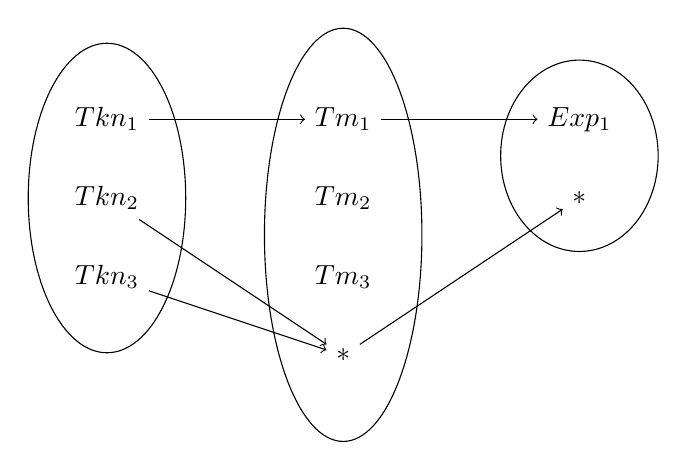
\begin{tikzpicture}
% Input Token
\node (Tkn1) at (0, 7) {$Tkn_1$};
\node[below of=Tkn1] (Tkn2) {$Tkn_2$};
\node[below of=Tkn2] (Tkn3) {$Tkn_3$};

% Output Term
\node (Tm1) at (3, 7) {$Tm_1$};
\node[below of=Tm1] (Tm2) {$Tm_2$};
\node[below of=Tm2] (Tm3) {$Tm_3$};
\node[below of=Tm3] (Nothing) {$\ast$};

% Output Exp
\node (Exp1) at (6, 7) {$Exp_1$};
\node[below of=Exp1] (Nothing2) {$\ast$};

% arrows
\path[->] (Tkn1) edge (Tm1);
\path[->] (Tkn2) edge (Nothing);
\path[->] (Tkn3) edge (Nothing);

\path[->] (Nothing) edge (Nothing2);
\path[->] (Tm1) edge (Exp1);

% set ellipses
\node[shape=ellipse,draw,minimum size=2cm,
      fit={(Tkn1) (Tkn3)}] {};
\node[shape=ellipse,draw,minimum size=2cm,
      fit={(Tm1) (Nothing)}] {};
\node[shape=ellipse,draw,minimum size=2cm,
      fit={(Exp1) (Nothing2)}] {};
\end{tikzpicture}
\end{frame}

\begin{frame}[fragile]
  \frametitle{Ideally, we'd like to restrict the domain.}
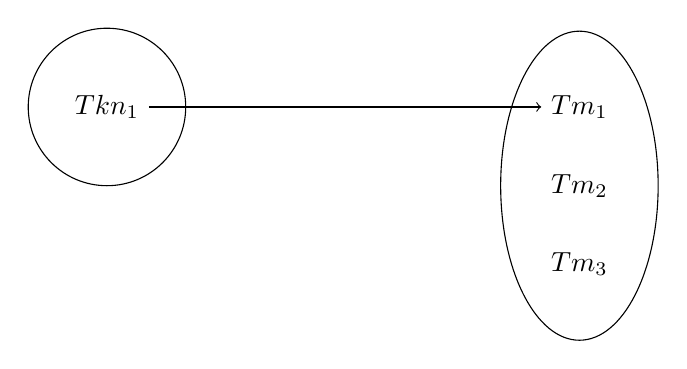
\begin{tikzpicture}
% Input Token
\node (Tkn1) at (0, 7) {$Tkn_1$};

% Output Term
\node (Tm1) at (6, 7) {$Tm_1$};
\node[below of=Tm1] (Tm2) {$Tm_2$};
\node[below of=Tm2] (Tm3) {$Tm_3$};


% arrows
\path[->] (Tkn1) edge (Tm1);

% set ellipses
\node[shape=ellipse,draw,minimum size=2cm,
      fit={(Tkn1) (Tkn1)}] {};
\node[shape=ellipse,draw,minimum size=2cm,
      fit={(Tm1) (Tm3)}] {};
\end{tikzpicture}
\\
Fortunately, we can do this via dependent types.
\end{frame}

\begin{frame}[fragile]
\frametitle{Indexing our valid tokens by tokens.}
\setbeamercolor{block title}{fg=white,bg=purple!75!black}
\setbeamercolor{block body}{fg=black,bg=white!80!gray}
\begin{block}{Token and ValidToken Types}
\begin{minted}{Idris}
data Token =
  TBigId
  | TSmallId
  | TArrow
  | TLambda
  | TNull

data ValidToken : Token -> Type where
  VTNull     : ValidToken TNull
  VTBigId    : ValidToken TBigId
  VTSmallId  : ValidToken TSmallId
  VTArrow    : ValidToken TArrow
  VTLambda   : ValidToken TLambda
\end{minted}
\end{block}
\end{frame}

\begin{frame}[fragile]
\frametitle{Indexing our valid tokens by tokens.}
\setbeamercolor{block title}{fg=white,bg=purple!75!black}
\setbeamercolor{block body}{fg=black,bg=white!80!gray}
\begin{block}{Token and ValidToken Types}
\begin{minted}{Idris}
-- null Token to satisfy totality checker.
total
match : String -> (a : Token ** ValidToken a)
match "foo" = (_ ** VTSmallId)
match "bar" = (_ ** VTSmallId)
match "baz" = (_ ** VTSmallId)
match "Foo" = (_ ** VTBigId)
match "=>"  = (_ ** VTArrow)
match "\\"  = (_ ** VTLambda)
match _     = (_ ** VTNull)
\end{minted}
\end{block}
\end{frame}

\begin{frame}[fragile]
\frametitle{An introduction to dependent pairs.}
\setbeamercolor{block title}{fg=white,bg=purple!75!black}
\setbeamercolor{block body}{fg=black,bg=white!80!gray}
\begin{block}{Dependant Pairs ($\Sigma$ types) in code.}
\begin{minted}{Idris}
data DPair : (a : Type) -> (a -> Type) -> Type
  MkDPair : {p : a -> Type}
         -> (fst : a) -> p fst -> DPair a p

fst : DPair a p -> a
fst (MkDPair x prf) = x

snd : {p : a -> Type}
   -> (rec : DPair a p) -> p (fst rec)
snd (MkDPair x prf) = prf
\end{minted}
\end{block}
\end{frame}

\begin{frame}[fragile]
\frametitle{Using dependent pairs and GADTs to restrict our
input domains.}
\setbeamercolor{block title}{fg=white,bg=purple!75!black}
\setbeamercolor{block body}{fg=black,bg=white!80!gray}
\begin{block}{Total Parsing with no maybes or errors}
\begin{minted}{Idris}
total
parseSmallId : ValidToken TSmallId -> Term
parseSmallId VTSmallId = MkRef

total 
example : Term
example = parseSmallId (DPair.snd (match "foo"))
\end{minted}
\end{block}
\end{frame}

\begin{frame}[fragile]
\frametitle{What about compositionality?}
\setbeamercolor{block title}{fg=white,bg=purple!75!black}
\setbeamercolor{block body}{fg=black,bg=white!80!gray}
\begin{block}{Dependent Function Composition}
\begin{minted}{Idris}
cm : {a : Type} 
 -> {b : a -> Type}
 -> {c : {x : a} -> b x -> Type}
 -> ({x : a} -> (y : b x) -> c y)
 -> (g : (x : a) -> b x)
 -> ((x : a) -> c (g x))
cm f g = \x => f (g x)

example2 : (x : String) 
        -> ValidToken (DPair.fst (match x))
example2 = (DPair.snd {p = ValidToken} `cm` match)
\end{minted}
\end{block}
\end{frame}

\begin{frame}[fragile]
\frametitle{Conclusions}
\setbeamercolor{block title}{fg=white,bg=green!75!black}
\setbeamercolor{block body}{fg=white,bg=green!25!black}
\begin{block}{Dependent Types can restrict our input domains.}
We saw how, using dependant pairs and GADTs, we may restrict
our input domains to be precisely the type we actually care
about, avoiding the need to wrap types in superfluous Eithers
and Maybes.
\end{block}
\setbeamercolor{block title}{fg=white,bg=orange!75!black}
\setbeamercolor{block body}{fg=white,bg=orange!25!black}
\begin{block}{Still not really compositional}
When types dependent on one-another it can be difficult to
compose them, even with dependent composition, due to the
dependency on the initial input. This suggests that dependent
types are less modular than 'plain' types (according to
Hughes) however there are other practical advantages to
dependent types.
\end{block}
\end{frame}

\end{document}
